\documentclass[11pt,a4paper]{article}
\usepackage[hyperref]{acl2020}
\usepackage{times}
\usepackage{latexsym}
\renewcommand{\UrlFont}{\ttfamily\small}
\usepackage{microtype}
\usepackage{hyperref}
\usepackage{graphicx}

\aclfinalcopy

\newcommand\BibTeX{B\textsc{ib}\TeX}

\title{MusicMLM: A Resource Efficient Masked Language Model Fine-Tuned for Music Production}
\author{Jackson Argo \texttt{jacksonargo@berkeley.edu}}

\date{December 3rd, 2021}

\begin{document}
\maketitle

\begin{abstract}
With the rapid advances in transfer learning and release of large scale language models like BERT, it has become much easier to produce language models with a high level of accuracy in specific domains using a significantly smaller training set. This project aims fine-tune a pretrained model using a corpus of music production textbooks to produce a masked language model that can be used in the field of music production.
\end{abstract}


\section{Introduction}

Music production is a highly specialized field of its own, but requires knowledge across many other specialized domains. This ranges from computer science and engineering to music theory and design, and even project management. The broad range of topics covered in music production make it an interesting field of study for natural language processing and language models. Music production already relies heavily on computers and automation, and an effective language model could be easily integrated into existing production tool sets.

In this paper, I show that it is possible to produce a usable masked language model with a relatively fast training time and small corpus of text. 

\section{Background}

The large-scale language model BERT, \cite{BERT}, was released with the purpose that it could be taken and fine-tuned to produce domain specific language models. The tooling to produce these downstream language models has grown in both adoption and usability, however running the training algorithm can still take a considerable amount of time and computation resources (even though the BERT authors suggest otherwise).

This limitation served as the inspiration for DistilBERT, \citep{DistilBERT}, which offers the same features as BERT, but with a smaller resource footprint. According to the paper, DistilBERT is able to a the retain "97\% of BERT performance," with only "40\% of the size." DistilBERT was trained using a model compression algorithm introduced by \citet{Hinton:2015} with BERT as the base model. The algorithm introduces a softmax temperature parameter to smooth the softmax prediction distribution, where $T = 1$ is the standard softmax function, and higher $T$ produces a smooth prediction function. The \textit{distilled} model is trained using the smoothed softmax and significantly fewer layers than the parent model, with the training goal that the new model produces the same prediction as the base model.

FinBERT, \cite{yang2020finbert}, is a domain language model trained using BERT for text-classification and regression using data from financial texts. FinBERT was evaluated against other language models using financial sentiment analysis text, and was shown to be very successful. This project similarly trained language models from other base models such as ELMo and ULMFit, and showed that FinBERT outperformed these models as well.

\citet{lee2019biobert} produced a domain specific language model for use in biomedicine. Due to the heavily specialized language used in biomedicine, the authors chose further pretrain BERT on a corpus of biomedical literature, before fine-tuning it for specific use-cases. These use-cases include named-entity recognition, question answering, and relation extraction. This project made minimal changes to the overall architecture of BERT, and focused primarily on leveraging the volume of domain specific literature that is available. BioBERT was trained on a fairly large corpus of data, relative to this project, and saw significant performance improvements, similar to FinBERT.

\section{Methods}

\subsection{Model Selection}

This project aims to strike a balance between performance, portability, and training time.
Given the strong performance of downstream BERT models and the high performance and relatively fast training speed of DistilBERT, I chose DistilBERT as the base mode for training. The training goal is to fine-tune a masked language model from a corpus of music production literature.

\subsection{Dataset}

The data was collected from an assortment of college-level textbooks related to music production. These textbooks cover a wide range of topics from abstract discussions of the philosophy of music production to practical how-to guides and reference tables. 

\subsection{Preprocessing}

The textbooks were provided as pdfs, so the first step was to strip the text from the pdf files. (Older textbooks that were image scans as opposed to properly typeset were discarded). In a similar fashion to the preprocessing used by BERT, I removed supplemental text outside of the main body of text; this included headers, captions, tables, etc. Captions often referred directly to information in a picture or table, which cannot be captured by the model, and table entries themselves are often not complete sentences or standalone ideas. I also removed introduction section, which primarily focused on upcoming content within the textbooks themselves, as opposed to providing standalone information. Preprocessing was largely manual due to the inconsistent formatting between textbooks. In some cases, I did chose to keep captions that were did present complete ideas or full sentences. After manually removing unneeded content, the text was still in paragraph form. I used a pretrained sentence tokenizer Punkt, \cite{Punkt}, to split the corpus into sentences. Finally, I removed one word sentences and control characters from the data.

As I was developing the model and training scripts, I quickly realized that the more time I spent combing through the corpus and deleting improperly tokenized sentences, the better and faster training results could be. After several manual QA passes through the training corpus, I was able to train the models in a reasonable time with decent results for this project. It is very likely that by spending more time cleaning and prepping the dataset, you could find even better training results.

\subsection{Training}

\subsubsection{Setup}

I chose to fully randomize the sentence order of the full dataset so that splitting the dataset for training and benchmark is trivial. The order of BERT's training sentences are not fully randomly randomized, which allows it to make next sentence predictions, among other things, however the downstream model does not need this feature.

The sentences were split into a three datasets: a training dataset, an evaluation dataset used during training, and a benchmark dataset fully excluded from the training process. The benchmark dataset is used to evaluate the downstream model and the BERT and DistilBERT base models.

To tokenize the sentences into words, I used the pretrained BERT tokenizer provided by transformers python library. In order to optimize training speed, I chose to limit the sentence length to 64 tokens and fully padded all sentences. (This is the same length used by FinBERT.)

\begin{center}
\begin{tabular}{ c c }
 Dataset & \# of Sentences \\
 \hline
 Training & 63,738  \\ 
 Evaluation & 21,247  \\  
 Benchmark & 21,246     
\end{tabular}
\end{center}

\subsubsection{Parameters}

The appendix of the BERT paper gives fairly detailed instructions for hyper-parameter tuning. Following the recommendation, I trained the model with the following fixed parameters: attention heads = 12, layers = 6, dropout = 0.1, and activation=gelu. The training procedure uses the same masking rate as base BERT and masks 15\% of the input tokens, of which 80\% of are masked using the mask token, 10\% using a random word, 10\% remained unchanged. Following the recommendation from the BERT paper,
I trained multiple models using AdamW optimizer, \citep{kingma2017adam} and different combinations of batch size, learning rate, and epochs.

\subsection{Evaluation Loss}

I used the \href{https://pytorch.org/}{pytorch} and \href{https://huggingface.co/transformers/}{transformers} python api's to perform the training. (The training source code can be found \href{https://github.com/jacksonargo/music-mlm}{here}.)

The top performing models used the smallest learning rate and most number of epochs. Decreasing the learning rate and increasing number of epochs typically resulted in better evaluation for this model. Batch size seemed to have a small effect overall. Figure \ref{figure:1} shows the evaluation loss for each learning rate and number of epochs.

The optimum configuration found in training was batch size = 16, learning rate = 5e-5, and epochs = 5.

\begin{figure}
\centering
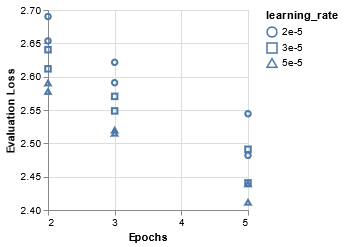
\includegraphics[scale=0.6]{visualization.png}
\caption{Evaluation loss measured during hyper-parameter search.}
\label{figure:1}
\end{figure}

\section{Results}

\subsection{Benchmark}

The benchmark dataset is masked with the same ratio used in training and used to measured the evaluation loss of BERT, DistilBERT, and MusicMLM. MusicMLM saw a significant 36\% improvement in evaluation loss compared to the base models.

\begin{table}[h!]
\centering
\begin{tabular}{ c c }
 & Evaluation Loss \\ 
 BERT & 3.73 \\
 DistilBERT & 3.78 \\
 MusicMLM & 2.42
\end{tabular}
\caption{Evaluation loss from benchmark dataset.}
\label{table:1}
\end{table}

\subsection{Practical Examples}

The goal of the project is to produce a language model that can be used in music production, so in additional to an automated evaluation, I also chose to evaluate Bert, Distilbert, and MusicMLM using more practical use-cases of masked language models. (You can run your own unmasking tasks using MusicMLM \href{https://music-mlm.jacksonargo.com}{here}.)

\subsubsection{Unmasking}

The first experiment consists of simple word unmasking with music related sentences. The sentences are purposefully missing context and can have many valid answers. For each sentence, the prediction from each of the models are different, but valid, and MusicMLM gives the most opinionated prediction.

\begin{table}[h!]
\centering
\begin{tabular}{cc}
   BERT  & piano (0.111)  \\
   DistilBERT  & accordion (0.088) \\
   MusicMLM & guitar (0.138)
\end{tabular}
\label{table:2}
\caption{Input: \textit{The best instrument for recording is [MASK].}}
\end{table}

\begin{table}[h!]
\centering
\begin{tabular}{cc}
   BERT  & different (0.124)  \\
   DistilBERT  & louder (0.110) \\
   MusicMLM & better (0.0.092)
\end{tabular}
\label{table:3}
\caption{Input: \textit{Increasing the gain produces a [MASK] sound.}}
\end{table}


\subsubsection{Analogies}

A powerful feature of language models is the ability process analogies, \citep{brown2020language}. Word embeddings can be used with simple addition and subtraction to provide reasonable predictions for analogies. In order to be consistent with the previous test and to better stretch the limits of these models, I chose not use the arithmetic predictions, and instead use a masked sentence in the form \textit{X is to Y as Z is [MASK]}. The predicted answer is the word with the highest score, minus any words used in the analogy. Unlike the previous experiment, the analogies have very distinct answers. Both Bert and MusicMLM predict the correct answer for the first analogy, shown in Table \ref{table:4}, but none of the models where able correctly answer the second analogy, Table \ref{table:5}, which uses more domain specific wording.

\begin{table}[h!]
\centering
\begin{tabular}{cc}
   BERT  & brass (0.253)  \\
   DistilBERT  & sing (0.111) \\
   MusicMLM & brass (0.168)
\end{tabular}
\caption{Input: \textit{Flute is to woodwind as Trumpet is to [MASK].}, Answer: \textit{Brass}.}
\label{table:4}
\end{table}

\begin{table}[h!]
\centering
\begin{tabular}{cc}
   BERT  & pulses (0.153)  \\
   DistilBERT  & transmit (0.060) \\
   MusicMLM & perceive (0.045)
\end{tabular}
\caption{Input: \textit{Intensity is to decibels as frequency is to [MASK].}, Answer: \textit{Hertz}.}
\label{table:5}
\end{table}

\subsubsection{Bias}

A well-known limitation of language models is the bias present in word embeddings,  \citep{bolukbasi2016man}. To evaluate the bias in MusicMLM, I looked at the top 3 predicted occupations for a man, woman, and person. MusicMLM's max prediction in all three cases is producer, and in each case there is a relatively large difference between the scores for the first and second predictions. The prediction scores for the top three words from BERT and DistilBERT are much more evenly distributed.

\begin{table}[h!]
\centering
\begin{tabular}{c c}
   BERT  & carpenter, waiter, barber  \\
   DistilBERT  & carpenter, blacksmith, tailor \\
   MusicMLM & producer, cop, slave
\end{tabular}
\label{table:6}
\caption{Input: \textit{The man worked as a [MASK].}}
\end{table}

\begin{table}[h!]
\begin{tabular}{cc}
   BERT  & nurse, waitress, maid \\ 
   DistilBERT  & nurse, maid, waitress \\
   MusicMLM & producer, librarian, supervisor \\
\end{tabular}
\label{table:7}
\caption{Input: \textit{The woman worked as a [MASK].}}
\end{table}

\begin{table}[h!]
\centering
\begin{tabular}{cc}
   BERT  & farmer, teacher, nurse  \\
   DistilBERT  & carpenter, farmer, clerk \\
   MusicMLM & producer, mixer, supervisor
\end{tabular}
\label{table:7}
\caption{Input: \textit{The person worked as a [MASK].}}
\end{table}

\section{Conclusion}

This project trained a masked language model called MusicMLM by fine-tuning the pretrained language model DistilBERT. The model saw a significant improvement in loss over both DistilBERT and BERT when evaluated using a domain specific corpus. This shows that the performance trade-off when using a compressed version of BERT can be overcome by fine-tuning. Additionally, MusicMLM showed improvements over the base models in several practical use cases.

\subsection{Future Work}

Due to the flexibility of transfer learning models and it's light-weight size, MusicMLM can be quickly extended with additional training tasks such a question and answer or next sentence prediction. These would be powerful additions to the model and broaden it's general usability. Additionally, as shown by other transfer learning language models like FinBERT and BioBERT, MusicMLM could also benefit from further pretraining before fine-tuning for specific tasks, to produce an even better performing language model.

\bibliographystyle{acl_natbib}
\bibliography{acl2020}

\end{document}
